%  LaTeX support: latex@mdpi.com 
%  For support, please attach all files needed for compiling as well as the log file, and specify your operating system, LaTeX version, and LaTeX editor.

%=================================================================
\documentclass[entropy,article,submit,pdftex,moreauthors]{Definitions/mdpi} 
%\documentclass[journal,article,submit,pdftex,moreauthors]{Definitions/mdpi}
%\documentclass[preprints,article,submit,pdftex,moreauthors]{Definitions/mdpi} 
% For posting an early version of this manuscript as a preprint, you may use "preprints" as the journal. Changing "submit" to "accept" before posting will remove line numbers.

% Below journals will use APA reference format:
% admsci, aieduc, behavsci, businesses, econometrics, economies, education, ejihpe, famsci, games, humans, ijcs, ijfs, journalmedia, jrfm, languages, psycholint, publications, tourismhosp, youth

% Below journals will use Chicago reference format:
% arts, genealogy, histories, humanities, jintelligence, laws, literature, religions, risks, socsci

%--------------------
% Class Options:
%--------------------
%----------
% journal
%----------
% Choose between the following MDPI journals:
% accountaudit, acoustics, actuators, addictions, adhesives, admsci, adolescents, aerobiology, aerospace, agriculture, agriengineering, agrochemicals, agronomy, ai, air, algorithms, allergies, alloys, amh, analytica, analytics, anatomia, anesthres, animals, antibiotics, antibodies, antioxidants, applbiosci, appliedchem, appliedmath, appliedphys, applmech, applmicrobiol, applnano, applsci, aquacj, architecture, arm, arthropoda, arts, asc, asi, astronomy, atmosphere, atoms, audiolres, automation, axioms, bacteria, batteries, bdcc, behavsci, beverages, biochem, bioengineering, biologics, biology, biomass, biomechanics, biomed, biomedicines, biomedinformatics, biomimetics, biomolecules, biophysica, biosensors, biosphere, biotech, birds, blockchains, bloods, blsf, brainsci, breath, buildings, businesses, cancers, carbon, cardiogenetics, catalysts, cells, ceramics, challenges, chemengineering, chemistry, chemosensors, chemproc, children, chips, cimb, civileng, cleantechnol, climate, clinbioenerg, clinpract, clockssleep, cmd, cmtr, coasts, coatings, colloids, colorants, commodities, complications, compounds, computation, computers, condensedmatter, conservation, constrmater, cosmetics, covid, crops, cryo, cryptography, crystals, csmf, ctn, curroncol, cyber, dairy, data, ddc, dentistry, dermato, dermatopathology, designs, devices, diabetology, diagnostics, dietetics, digital, disabilities, diseases, diversity, dna, drones, dynamics, earth, ebj, ecm, ecologies, econometrics, economies, education, eesp, ejihpe, electricity, electrochem, electronicmat, electronics, encyclopedia, endocrines, energies, eng, engproc, ent, entomology, entropy, environments, epidemiologia, epigenomes, esa, est, famsci, fermentation, fibers, fintech, fire, fishes, fluids, foods, forecasting, forensicsci, forests, fossstud, foundations, fractalfract, fuels, future, futureinternet, futureparasites, futurepharmacol, futurephys, futuretransp, galaxies, games, gases, gastroent, gastrointestdisord, gastronomy, gels, genealogy, genes, geographies, geohazards, geomatics, geometry, geosciences, geotechnics, geriatrics, glacies, grasses, greenhealth, gucdd, hardware, hazardousmatters, healthcare, hearts, hemato, hematolrep, heritage, higheredu, highthroughput, histories, horticulturae, hospitals, humanities, humans, hydrobiology, hydrogen, hydrology, hygiene, idr, iic, ijerph, ijfs, ijgi, ijmd, ijms, ijns, ijpb, ijt, ijtm, ijtpp, ime, immuno, informatics, information, infrastructures, inorganics, insects, instruments, inventions, iot, j, jal, jcdd, jcm, jcp, jcs, jcto, jdad, jdb, jeta, jfb, jfmk, jimaging, jintelligence, jlpea, jmahp, jmmp, jmms, jmp, jmse, jne, jnt, jof, joitmc, joma, jop, jor, journalmedia, jox, jpbi, jpm, jrfm, jsan, jtaer, jvd, jzbg, kidney, kidneydial, kinasesphosphatases, knowledge, labmed, laboratories, land, languages, laws, life, lights, limnolrev, lipidology, liquids, literature, livers, logics, logistics, lubricants, lymphatics, machines, macromol, magnetism, magnetochemistry, make, marinedrugs, materials, materproc, mathematics, mca, measurements, medicina, medicines, medsci, membranes, merits, metabolites, metals, meteorology, methane, metrics, metrology, micro, microarrays, microbiolres, microelectronics, micromachines, microorganisms, microplastics, microwave, minerals, mining, mmphys, modelling, molbank, molecules, mps, msf, mti, multimedia, muscles, nanoenergyadv, nanomanufacturing, nanomaterials, ncrna, ndt, network, neuroglia, neurolint, neurosci, nitrogen, notspecified, nursrep, nutraceuticals, nutrients, obesities, oceans, ohbm, onco, oncopathology, optics, oral, organics, organoids, osteology, oxygen, parasites, parasitologia, particles, pathogens, pathophysiology, pediatrrep, pets, pharmaceuticals, pharmaceutics, pharmacoepidemiology, pharmacy, philosophies, photochem, photonics, phycology, physchem, physics, physiologia, plants, plasma, platforms, pollutants, polymers, polysaccharides, populations, poultry, powders, preprints, proceedings, processes, prosthesis, proteomes, psf, psych, psychiatryint, psychoactives, psycholint, publications, purification, quantumrep, quaternary, qubs, radiation, reactions, realestate, receptors, recycling, regeneration, religions, remotesensing, reports, reprodmed, resources, rheumato, risks, robotics, rsee, ruminants, safety, sci, scipharm, sclerosis, seeds, sensors, separations, sexes, signals, sinusitis, siuj, skins, smartcities, sna, societies, socsci, software, soilsystems, solar, solids, spectroscj, sports, standards, stats, std, stresses, surfaces, surgeries, suschem, sustainability, symmetry, synbio, systems, tae, targets, taxonomy, technologies, telecom, test, textiles, thalassrep, therapeutics, thermo, timespace, tomography, tourismhosp, toxics, toxins, transplantology, transportation, traumacare, traumas, tropicalmed, universe, urbansci, uro, vaccines, vehicles, venereology, vetsci, vibration, virtualworlds, viruses, vision, waste, water, wem, wevj, wild, wind, women, world, youth, zoonoticdis

%---------
% article
%---------
% The default type of manuscript is "article", but can be replaced by: 
% abstract, addendum, article, benchmark, book, bookreview, briefcommunication, briefreport, casereport, changes, clinicopathologicalchallenge, comment, commentary, communication, conceptpaper, conferenceproceedings, correction, conferencereport, creative, datadescriptor, discussion, entry, expressionofconcern, extendedabstract, editorial, essay, erratum, fieldguide, hypothesis, interestingimages, letter, meetingreport, monograph, newbookreceived, obituary, opinion, proceedingpaper, projectreport, reply, retraction, review, perspective, protocol, shortnote, studyprotocol, supfile, systematicreview, technicalnote, viewpoint, guidelines, registeredreport, tutorial,  giantsinurology, urologyaroundtheworld
% supfile = supplementary materials

%----------
% submit
%----------
% The class option "submit" will be changed to "accept" by the Editorial Office when the paper is accepted. This will only make changes to the frontpage (e.g., the logo of the journal will get visible), the headings, and the copyright information. Also, line numbering will be removed. Journal info and pagination for accepted papers will also be assigned by the Editorial Office.

%------------------
% moreauthors
%------------------
% If there is only one author the class option oneauthor should be used. Otherwise use the class option moreauthors.

%---------
% pdftex
%---------
% The option pdftex is for use with pdfLaTeX. Remove "pdftex" for (1) compiling with LaTeX & dvi2pdf (if eps figures are used) or for (2) compiling with XeLaTeX.

%=================================================================
% MDPI internal commands - do not modify
\firstpage{1} 
\makeatletter 
\setcounter{page}{\@firstpage} 
\makeatother
\pubvolume{1}
\issuenum{1}
\articlenumber{0}
\pubyear{2025}
\copyrightyear{2025}
%\externaleditor{Firstname Lastname} % More than 1 editor, please add `` and '' before the last editor name
\datereceived{ } 
\daterevised{ } % Comment out if no revised date
\dateaccepted{ } 
\datepublished{ } 
%\datecorrected{} % For corrected papers: "Corrected: XXX" date in the original paper.
%\dateretracted{} % For retracted papers: "Retracted: XXX" date in the original paper.
\hreflink{https://doi.org/} % If needed use \linebreak
%\doinum{}
%\pdfoutput=1 % Uncommented for upload to arXiv.org
%\CorrStatement{yes}  % For updates
%\longauthorlist{yes} % For many authors that exceed the left citation part

%=================================================================
% Add packages and commands here. The following packages are loaded in our class file: fontenc, inputenc, calc, indentfirst, fancyhdr, graphicx, epstopdf, lastpage, ifthen, float, amsmath, amssymb, lineno, setspace, enumitem, mathpazo, booktabs, titlesec, etoolbox, tabto, xcolor, colortbl, soul, multirow, microtype, tikz, totcount, changepage, attrib, upgreek, array, tabularx, pbox, ragged2e, tocloft, marginnote, marginfix, enotez, amsthm, natbib, hyperref, cleveref, scrextend, url, geometry, newfloat, caption, draftwatermark, seqsplit
% cleveref: load \crefname definitions after \begin{document}
\usepackage{physics}

%=================================================================
% Please use the following mathematics environments: Theorem, Lemma, Corollary, Proposition, Characterization, Property, Problem, Example, ExamplesandDefinitions, Hypothesis, Remark, Definition, Notation, Assumption
%% For proofs, please use the proof environment (the amsthm package is loaded by the MDPI class).

%=================================================================
% Full title of the paper (Capitalized)
\Title{Entropy of the cell fluid model with Curie-Weiss interation}

% MDPI internal command: Title for citation in the left column
\TitleCitation{Entropy of the cell fluid model with Curie-Weiss interaction}

% Author Orchid ID: enter ID or remove command
\newcommand{\orcidauthorA}{0009-0008-2405-9038} % Add \orcidA{} behind the author's name
%\newcommand{\orcidauthorB}{0000-0000-0000-000X} % Add \orcidB{} behind the author's name

% Authors, for the paper (add full first names)
\Author{R.~V. Romanik $^{1,}$*\orcidA{}, O.~A. Dobush, M.~P. Kozlovskii, I.~V. Pylyuk, M.~A. Shpot}

%\longauthorlist{yes}

% MDPI internal command: Authors, for metadata in PDF
\AuthorNames{R.~V. Romanik, O.~A. Dobush, M.~P. Kozlovskii, I.~V. Pylyuk, M.~A. Shpot}

% MDPI internal command: Authors, for citation in the left column, only choose below one of them according to the journal style
% If this is a Chicago style journal 
% (arts, genealogy, histories, humanities, jintelligence, laws, literature, religions, risks, socsci): 
% Lastname, Firstname, Firstname Lastname, and Firstname Lastname.

% If this is a APA style journal 
% (admsci, behavsci, businesses, econometrics, economies, education, ejihpe, games, humans, ijfs, journalmedia, jrfm, languages, psycholint, publications, tourismhosp, youth): 
% Lastname, F., Lastname, F., \& Lastname, F.

% If this is a ACS style journal (Except for the above Chicago and APA journals, all others are in the ACS format): 
% Lastname, F.; Lastname, F.; Lastname, F.
\isAPAStyle{%
       \AuthorCitation{Romanik, R.V., Dobush, O.~A., Kozlovskii, M.~P., Pylyuk, I.~V., \& Shpot, M.~A.}
         }{%
        \isChicagoStyle{%
        \AuthorCitation{Lastname, Firstname, Firstname Lastname, and Firstname Lastname.}
        }{
        \AuthorCitation{Romanik, R.V.; Dobush, O.~A.; Kozlovskii, M.~P.; Pylyuk, I.~V.; \& Shpot, M.~A.}
        }
}

% Affiliations / Addresses (Add [1] after \address if there is only one affiliation.)
\address[1]{%
$^{1}$ \quad Yukhnovskii Institute for Condensed Matter Physics of NAS of Ukraine; Lviv, Ukraine\\
%$^{2}$ \quad Affiliation 2; e-mail@e-mail.com
}

% Contact information of the corresponding author
\corres{Correspondence: romanik@icmp.lviv.ua;}

% Current address and/or shared authorship
%\firstnote{Current address: Affiliation.}  
% Current address should not be the same as any items in the Affiliation section.

%\secondnote{These authors contributed equally to this work.}
% The commands \thirdnote{} till \eighthnote{} are available for further notes.

%\simplesumm{} % Simple summary

%\conference{} % An extended version of a conference paper

% Abstract (Do not insert blank lines, i.e. \\) 
\abstract{Entropy of the cell fluid model with Curie-Weiss interaction is obtained in analytical form as a function of temperature and chemical potential.
A parametric equation is derived representing the entropy as a function of density. Features of both the entropy per particle and the entropy per cell are investigated at the ``entropy-density'' and ``entropy-chemical potential'' planes. The considered cell model is a multiple-occupancy model and possesses an infinite sequence of first-order phase transitions at sufficiently low temperature. We found that the entropy exhibits profound minima at around integer-valued particle densities, which may be a generic feature of multiple-occupancy models.}

% Keywords
\keyword{Entropy; lattice model; multiple occupancy} 

% The fields PACS, MSC, and JEL may be left empty or commented out if not applicable
%\PACS{J0101}
%\MSC{}
%\JEL{}

%%%%%%%%%%%%%%%%%%%%%%%%%%%%%%%%%%%%%%%%%%
% Only for the journal Diversity
%\LSID{\url{http://}}

%%%%%%%%%%%%%%%%%%%%%%%%%%%%%%%%%%%%%%%%%%
% Only for the journal Applied Sciences
%\featuredapplication{Authors are encouraged to provide a concise description of the specific application or a potential application of the work. This section is not mandatory.}
%%%%%%%%%%%%%%%%%%%%%%%%%%%%%%%%%%%%%%%%%%

%%%%%%%%%%%%%%%%%%%%%%%%%%%%%%%%%%%%%%%%%%
% Only for the journal Data
%\dataset{DOI number or link to the deposited data set if the data set is published separately. If the data set shall be published as a supplement to this paper, this field will be filled by the journal editors. In this case, please submit the data set as a supplement.}
%\datasetlicense{License under which the data set is made available (CC0, CC-BY, CC-BY-SA, CC-BY-NC, etc.)}

%%%%%%%%%%%%%%%%%%%%%%%%%%%%%%%%%%%%%%%%%%
% Only for the journal BioTech, Fishes, Neuroimaging and Toxins
%\keycontribution{The breakthroughs or highlights of the manuscript. Authors can write one or two sentences to describe the most important part of the paper.}

%%%%%%%%%%%%%%%%%%%%%%%%%%%%%%%%%%%%%%%%%%
% Only for the journal Encyclopedia
%\encyclopediadef{For entry manuscripts only: please provide a brief overview of the entry title instead of an abstract.}

%%%%%%%%%%%%%%%%%%%%%%%%%%%%%%%%%%%%%%%%%%
% Only for the journal Advances in Respiratory Medicine, Future, Sensors and Smart Cities
%\addhighlights{yes}
%\renewcommand{\addhighlights}{%
%
%\noindent This is an obligatory section in ``Advances in Respiratory Medicine'', ``Future'', ``Sensors'' and ``Smart Cities”, whose goal is to increase the discoverability and readability of the article via search engines and other scholars. Highlights should not be a copy of the abstract, but a simple text allowing the reader to quickly and simplified find out what the article is about and what can be cited from it. Each of these parts should be devoted up to 2~bullet points.\vspace{3pt}\\
%\textbf{What are the main findings?}
% \begin{itemize}[labelsep=2.5mm,topsep=-3pt]
% \item First bullet.
% \item Second bullet.
% \end{itemize}\vspace{3pt}
%\textbf{What is the implication of the main finding?}
% \begin{itemize}[labelsep=2.5mm,topsep=-3pt]
% \item First bullet.
% \item Second bullet.
% \end{itemize}
%}

%%%%%%%%%%%%%%%%%%%%%%%%%%%%%%%%%%%%%%%%%%
\begin{document}

%%%%%%%%%%%%%%%%%%%%%%%%%%%%%%%%%%%%%%%%%%
%\setcounter{section}{-1} %% Remove this when starting to work on the template.

\section{Introduction}

Lattice-gas models that allow multiple occupancy of a cell, in contrast to classical lattice gases~\citep{LY52,Stanley71} where each cell can contain at most one particle, have been studied much less frequently. Nevertheless, they represent a valuable class of models capable of reproducing the essential thermodynamic features of fluids with soft or penetrable interactions~\citep{Stillinger76,LWL98,FHL04,FL18,LYZ21}. From the statistical-mechanical point of view, such systems constitute an interesting theoretical object that exhibits nontrivial collective behavior while remaining analytically tractable within mean-field or Curie–Weiss-type approximations~\citep{KKD20,KD22}.

Among the thermodynamic quantities characterizing these systems, entropy plays a central role, as it provides a direct measure of configurational degeneracy and is closely related to the onset of phase transitions. Although some studies~\citep{dOG78,FHL04,Prestipino14,PGT15,FL18,LYZ21,KD22} have addressed the thermodynamic and phase properties of multi-occupancy models, their entropic characteristics remain largely unexplored. In the present work, we aim to address this gap by deriving explicit analytical expressions for the entropy of a cell fluid model with multiple occupancy and Curie–Weiss-type attraction. Because of its mean-field character, the Curie–Weiss interaction allows for an exact thermodynamic solution, making it a convenient analytical reference for multi-occupancy systems.

Following Stanley~\citep[Appendix A]{Stanley71}, we interpret the lattice gas as a cell fluid, that is, as a system in which a particle center is located in a cell and particle positions are not restricted to a discrete set of sites in a lattice. In our case, each cell may contain an arbitrary number of particles, and the  interaction is defined through both short-range repulsion and long-range mean-field attraction. The present study extends the results of~~\citep{KKD20,KD22,RDKPS25arxiv} by focusing on the entropy and its dependence on chemical potential, particle density, and temperature.

The paper is organized as follows. In Section~\ref{sec:model}, the model is briefly described. Section~\ref{sec:res} presents exact entropy expressions, and illustrates the results numerically and graphically, while their physical interpretation and qualitative similarity with other systems are discussed in~Section~\ref{sec:dis}.

%%%%%%%%%%%%%%%%%%%%%%%%%%%%%%%%%%%%%%%%%%
\section{Model and Definitions}
\label{sec:model}
An open system of point particles is considered in volume $V\subset\mathbb R^3$ in three space dimensions. The total volume $V$ is partitioned into $N_v$ non-overlapping congruent cubic cells $\Delta_l$, $l\in\{1,...,N_v\}$, each of volume $v$, such that $V$ is the union of all $\Delta_l$'s:
\begin{equation}\label{volume}
	V = \bigcup_{l=1}^{N_v}\Delta_l,\qquad
	\Delta_l \cap \Delta_{l'} = \emptyset, \text{ if } l \neq l',\qquad\mbox{and}\quad
	V = v N_v.
\end{equation}
The two-particle interaction is defined as
\begin{equation}
	\label{def:curie-weiss-pot}
	\Phi_{N_v}(\vb{r}_i, \vb{r}_j) = -\frac{J_1}{N_v} + J_2\sum_{l=1}^{N_v} \mathbb{I}_{\Delta_l}(\vb{r}_i) \mathbb{I}_{\Delta_l}(\vb{r}_j).
\end{equation}
The first term in $\Phi_{N_v}$ describes a global Curie-Weiss (mean-field-like) attraction for any pair of particles in the system.
The strength of this attraction is controlled by an energy parameter $J_1 > 0$. The second term in $\Phi_{N_v}$ describes a local repulsion between two particles contained within the same cell $\Delta_l$ and is characterized by the parameter $J_2 > 0.$
Here, $\mathbb{I}_{\Delta_l}(\vb{r})$ is the indicator function of a cell $\Delta_l$,
\begin{equation}
	\label{def:I}
	\mathbb{I}_{\Delta_l} (\vb{r}) = \left\{
	\begin{array}{ll}
		1, \quad \vb{r} \in \Delta_l,
		\\
		0, \quad \vb{r} \notin \Delta_l.
	\end{array}
	\right.
\end{equation}
We refer the reader to Refs.~\citep{KKD20,KD22,RDKPS25arxiv} for a more rigorous definition of the model. The main features of the model are the following:
\begin{itemize}
	\item the model possesses an exact solution in the thermodynamic limit;
	
	\item for sufficiently low temperatures, the model exhibits an infinite sequence of first-order phase transitions between fluid phases of ever increasing density;
	
	\item the phase transition lines between each pair of neighboring (adjacent) phases end with a respective critical point, and therefore an infinite number of critical points exist in the model.
	
\end{itemize}
The phase diagrams in both the temperature-density and pressure-temperature planes are presented in~\citep{KD22}.

One of the main results of~\citep{RDKPS25arxiv} is the explicit expressions for the entropy of the model as a function of temperature and chemical potential. In the next Section~\ref{sec:res}, we thoroughly analyze the these expressions for the entropy in detail. 

We use the following standard dimensionless variables: the reduced temperature $T^*=k_{\rm B}T/J_1$, the reduced pressure $P^* = P v/J_1$, the reduced chemical potential $\mu^* = \mu/J_1$, the reduced particle density $\rho^* = \frac{\langle N \rangle}{V} v = \frac{\langle N \rangle}{N_v}$, with $T$ being the absolute temperature, $k_{\rm B}$ the Boltzmann constant, $P$ the pressure, $\mu$ the chemical potential, and $\langle N \rangle$ the average number of particles, where the brackets denote a grand-canonical ensemble average. For the entropy $S$, the corresponding reduced quantity is
\begin{equation}
	\label{def:S1}
	S^* = \frac{S}{k_{\rm B} \langle N \rangle}.
\end{equation}
We call $S^*$ the \textit{entropy per particle}. For lattice models, the \textit{entropy per cell} (or the \textit{entropy per site}) $S^*_v$ is also defined as
\begin{equation}
	\label{def:S2}
	S^*_v = \frac{S}{k_{\rm B} N_v}.
\end{equation}
The thermodynamic formula for the entropy per particle is
\begin{eqnarray}
	S^* & = & \frac{1}{\rho^*}\left(\frac{\partial P^*}{\partial T^*}\right)_{{\mu^*}}
	= \frac{(\partial P^* / \partial T^*)_{{\mu^*}}}{(\partial P^* / \partial \mu^*)_{T^*}}.
\end{eqnarray}
Using Eqs.~\eqref{def:S1} and \eqref{def:S2}, the corresponding entropy per cell is
\begin{equation}
	S^*_v = \rho^* S^* = \left(\frac{\partial P^*}{\partial T^*}\right)_{\mu^*}.
\end{equation}


%%%%%%%%%%%%%%%%%%%%%%%%%%%%%%%%%%%%%%%%%%
\section{Results}\label{sec:res}
From~\citep{RDKPS25arxiv}, the reduced entropy per particle can be written in the analytical form
\begin{equation}
	\label{eq:entropy1}
	S^*(T^*,\mu^*) = \left(\frac{3}{2} - \frac{\mu^*}{T^*}\right) - \frac{1}{T^*}\frac{K_1}{K_0} + \frac{K_0 \ln K_0}{K_1} + \frac{a}{2T^*} \frac{K_2}{K_1},
\end{equation}
where $a = J_2/J_1$, and the special functions $K_j$, with $j=0, 1, 2, \ldots$, are themselves functions of temperature $T^*$ and chemical potential $\mu^*$:
\begin{equation}
	\label{def:Kj}
	K_j(T^*,\mu^*;\bar{y}_{\rm max}) = \sum_{n=0}^{\infty} \frac{n^j (v^* T^{*3/2})^n}{n!} \exp[\left(\bar{y}_{\rm max}+\frac{\mu^*}{T^*}\right)n - \frac{a}{2T^*}n^2].
\end{equation}
Here $v^* = v/\lambda^3$, $\lambda = (2\pi\hbar^2/mJ_1)^{1/2}$, with $\hbar$ the Planck constant, $m$ the mass of a particle. A quantity analogous to $v^*$ appears in~\citep{PGT15} in the context of a model that also allows for multiple occupancy.

The quantity $\bar{y}_{\rm max}$ in \eqref{def:Kj} is itself a function of $T^*$ and $\mu^*$, and we just simplify notation by implying $\bar{y}_{\mathrm{max}} = \bar{y}_{\mathrm{max}}(T^*,\mu^*)$. It is determined from the extremum condition
\begin{eqnarray}
	\label{cond:max}
	E_1(T^*,\mu^*; \bar{y}_{\rm max}) & = & 0,
	\nonumber\\
	E_2(T^*,\mu^*;\bar{y}_{\rm max}) & < & 0,
\end{eqnarray}
with functions $E_1$ and $E_2$ defined as
\begin{equation}
	\label{def:E1}
	E_1(T^*,\mu^*;y) = -T^* y + \frac{K_1(T^*,\mu^*;y)}{K_0(T^*,\mu^*;y)};
\end{equation}
\begin{equation}
	E_2(T^*,\mu^*;y) = -T^*+\frac{K_2(T^*,\mu^*;y)}{K_0(T^*,\mu^*;y)}
	-\left[\frac{K_1(T^*,\mu^*;y)}{K_0(T^*,\mu^*;y)}\right]^2\!.
\end{equation}

When the ideal-gas contribution to the chemical potential, $\mu_{\rm{id}} = k_{\rm{B}}T \ln(N\Lambda^3/V)$, is taken into account, it becomes evident that the first term in~\eqref{eq:entropy1} 
\begin{equation}
	S^*_{\rm id} = \frac{3}{2} - \frac{\mu^*}{T^*}
\end{equation}
represents the entropy of a system of noninteracting molecules arranged on a lattice, subject to the strict single-occupancy constraint (one particle per cell), see~\citep[(47.4)]{Hill56}.

The explicit formula for the entropy per cell is
\begin{eqnarray}
	\label{eq:entropy2}
	S^{*}_v(T^*,\mu^*) & = & \left(\frac{3}{2} - \frac{\mu^*}{T^*}\right)\frac{K_1}{K_0} - \frac{1}{T^*}\frac{K_1^2}{K_0^2} + \ln K_0 + \frac{a}{2T^*} \frac{K_2}{K_0}.
\end{eqnarray}
Equations~\eqref{eq:entropy1} and~\eqref{eq:entropy2} express the entropy as a function of temperature and chemical potential. To obtain the entropy dependence on the density $\rho^*$, we should account for the following equation \citep[(42)]{RDKPS25arxiv}:
\begin{equation}
	\label{eq:rho_in_y}
	\rho^*=\frac{K_1(T^*,\mu^*;\bar{y}_{\rm max})}{K_0(T^*,\mu^*;\bar{y}_{\rm max})}.
\end{equation}

%\subsection{Parametric representation}
Let us now represent the analytical results for entropy in the form of parametric equations. Noticing that by~\eqref{cond:max} and~\eqref{def:E1}
\begin{equation}
	\bar{y}_{\rm max} = \frac{1}{T^*}\frac{K_1(T^*,\mu^*;y)}{K_0(T^*,\mu^*;y)}
\end{equation}
and applying the idea taken from~\citep{KD22}, we introduce a new function
\begin{equation}
	\bar{z}_{\rm max}(T^*,\mu^*) = \bar{y}_{\rm max} + \frac{\mu^*}{T^*},
\end{equation}
and rewrite the entropy in the form
\begin{equation}
	\label{eq:S_in_z}
	S^*(T^*;\bar{z}_{\rm max}) = \frac{3}{2} - \bar{z}_{\rm max} + \frac{\tilde{K}_0 \ln \tilde{K}_0}{\tilde{K}_1} + \frac{a}{2T^*} \frac{\tilde{K}_2}{\tilde{K}_1},
\end{equation}
where the special functions $\tilde{K}_j$ are now written as
\begin{equation}
	\tilde{K}_j(T^*;\bar{z}_{\rm max}) = \sum_{n=0}^{\infty} \frac{n^j (v^* T^{*3/2})^n}{n!} \exp[\bar{z}_{\rm max}n - \frac{a}{2T^*}n^2].
\end{equation}
The chemical potential is expressed in $\tilde{K}_j$ as
\begin{equation}
	\label{eq:mu_in_z}
	\mu^* = T^* \bar{z}_{\rm max} - \frac{\tilde{K}_1(T^*;\bar{z}_{\rm max})}{\tilde{K}_0(T^*;\bar{z}_{\rm max})}.
\end{equation}
At any given temperature $T^*$, Eqs.~\eqref{eq:S_in_z} and~\eqref{eq:mu_in_z} can be formally considered as a parametric equation for the entropy $S^*$ as a function of $\mu^*$, with $\bar{z}_{\rm max}$ being the parameter.

Similarly, if Eq.~\eqref{eq:rho_in_y} is rewritten as
\begin{equation}
	\label{eq:rho_in_z}
	\rho^*(T^*;\bar{z}_{\rm max}) = \frac{\tilde{K}_1(T^*;\bar{z}_{\rm max})}{\tilde{K}_0(T^*;\bar{z}_{\rm max})},
\end{equation}
then Eqs.~\eqref{eq:S_in_z} and~\eqref{eq:rho_in_z} constitute a parametric equation for the entropy $S^*$ as a function of $\rho^*$, at any given $T^*$ and with $\bar{z}_{\rm max}$ being the parameter.
The explicit expression for the entropy per cell in terms of $\bar{z}_{\mathrm{max}}$ and $\tilde{K}_j$ reads
\begin{equation}
	\label{eq:S2_in_z}
	S^*_v(T^*;\bar{z}_{\rm max}) = \left(\frac{3}{2} - \bar{z}_{\rm max}\right) \frac{\tilde{K}_1}{\tilde{K}_0} + \ln \tilde{K}_0 + \frac{a}{2T^*} \frac{\tilde{K}_2}{\tilde{K}_0},
\end{equation}


\begin{table}
	\caption{Critical point coordinates for the first four critical points of the cell fluid model with Curie-Weiss interaction. All numerical calculations were performed for $a=1.2$ and $v^*=5.0$.}
	\label{tab1}
	%\begin{adjustwidth}{-\extralength}{0cm}
		\begin{tabularx}{\textwidth}{CCCCCCC}
			$n$ & $T^*_c$ & $\rho^*_c$ & $\mu^*_c$ & $S^*_c$ & $S^*_{v, c}$ & $\bar{z}_c$ \\
			\midrule
			
			1 & 0.254567 & 0.513896 & 0.209380 & 2.43173 & 1.24966 & 2.84119 \\
			\midrule
			2 & 0.261881 & 1.50557 & 0.585097 & 1.34933 & 2.03151 & 7.98327 \\
			
			\midrule
			3 & 0.265254 & 2.50303 & 0.891843 & 0.914901 & 2.29002 & 12.7985 \\
			
			\midrule
			4 & 0.267242 & 3.50191 & 1.16893 & 0.631157 & 2.21025 & 17.4779 \\
			
			\bottomrule
		\end{tabularx}		
	%\end{adjustwidth}
\end{table}

Before proceeding with analysis of the entropy behavior, let us recall that the considered model possesses an infinite number of critical points, and thus, an infinite number of first-order phase transitions at sufficiently low temperatures~\citep{KD22}. We call the phase with the lowest density Phase I. Then the first first-order phase transition leads to a phase with a higher density, Phase II. The second first-order phase transition results in Phase III, and so on to Phase IV, Phase V, etc. Phase diagrams in the temperature-density plane is shown in~\citep[Fig.~10]{KD22}, detailed numerical values of quantities at the first five critical points are summarized in \citep[Table~1]{RDKPS25arxiv}. For reference, Table~\ref{tab1} lists the critical values of relevant physical quantities for the first four critical points, and Table~\ref{tab2} presents their values at the coexistence lines at temperatures $T^*=0.25$ and $T^*=0.20$. 

\begin{table}[H]
	\caption{Coexistence-line values for some quantities. All numerical calculations were performed for $a=1.2$ and $v^*=5.0$.\label{tab2}}
	\begin{adjustwidth}{-\extralength}{0cm}
		\begin{tabularx}{\fulllength}{C|C|CCCCCCC}
		Coexisting phases	&$T^*$	& $\mu^*_{I-II}$	& $\rho^*_I$   & $\rho^*_{II}$ & $S^*_{I}$ & $S^*_{II}$ & $\bar{z}_{I}$ & $\bar{z}_{II}$ \\
			\midrule
			\multirow[m]{2}{*}{I - II} &
			0.25 & 0.214259 & 0.397996 & 0.628565 & 2.73453 & 2.11856 & 2.44902 & 3.37130 \\
			&0.20 & 0.259145 & 0.142070 & 0.871833 & 3.57349 & 1.18911 & 2.00607 & 5.65489 \\
			
			\midrule
				& & $\mu^*_{II-III}$	& $\rho^*_{II}$   & $\rho^*_{III}$ & $S^*_{II}$ & $S^*_{III}$ & $\bar{z}_{II}$ & $\bar{z}_{III}$ \\
			\midrule
			\multirow[m]{2}{*}{II - III}
			& 0.25 & 0.589630 & 1.32372 & 1.68613 & 1.36451 & 1.14578 & 7.65338 & 9.10305 \\
			& 0.20 & 0.598952 & 1.12438 & 1.88058 & 0.996714 & 0.601031 & 8.61664 & 12.3977 \\
			
			\midrule
			& & $\mu^*_{III-IV}$	& $\rho^*_{III}$   & $\rho^*_{IV}$ & $S^*_{III}$ & $S^*_{IV}$ & $\bar{z}_{III}$ & $\bar{z}_{IV}$ \\
			\midrule
			\multirow[m]{2}{*}{III - IV}
			& 0.25 & 0.891559 & 2.29983 & 2.70532 & 0.874317 &0.733783 & 12.7655 & 14.3875 \\
			& 0.20 & 0.880351 & 2.11796 & 2.88459 & 0.510408 & 0.269009 & 14.9915 & 18.8247 \\
			
			\midrule
			& & $\mu^*_{IV-V}$	& $\rho^*_{IV}$   & $\rho^*_{V}$ & $S^*_{IV}$ & $S^*_{V}$ & $\bar{z}_{IV}$ & $\bar{z}_{V}$\\
			\midrule
			\multirow[m]{2}{*}{IV - V}
			& 0.25 & 1.16371 & 3.28767 & 3.71550 & 0.565479 & 0.459722 & 17.8055 & 19.5168 \\
			& 0.20 & 1.13801 & 3.11462 & 3.88693 & 0.208441 & 0.0303822 & 21.2632 & 25.1247 \\
			
			\bottomrule
		\end{tabularx}
	\end{adjustwidth}
\end{table}


The analytical results for the entropy are visualized in Figure~\ref{fig:entropy3}. Panels (a) and (b) illustrate the entropy per particle, while panels (c) and (d) correspond to the entropy per cell.
The numerical values for the parameters are taken as $a=1.2$, and $v^*=5.0$. Each panel in Figure~\ref{fig:entropy3} shows four temperature curves: the red curve is $T^* = 0.4$, which is much higher than the critical temperatures; the green curve is $T^* = 0.3$, which is slightly higher than the critical temperatures; the black curve is $T^*=0.25$, which is just slightly lower than the critical temperatures; and the blue curve is $T^*=0.20$, which is significantly lower than the critical temperatures. The solid parts of the curves represent the results for the stable phases, while the dashed parts correspond to two-phase regions, i.e. to solutions of $\bar{y}$ to $E_1=0$ that may violate the condition of global maxima $E_2 < 0$, see~\eqref{cond:max}. 

The dependence of the entropy per particle on the chemical potential is presented in Figure~\ref{fig:entropy3}(a). For the supercritical region, red and green curves, the entropy $S^*$ has a monotonic decreasing behavior with the chemical potential $\mu^*$. For temperatures below the critical ones, we observe that phase II has a lower entropy than Phase I. Consequently, Phase III has a lower entropy than Phase II, and so on. However, within a particular phase, except Phase I, the dependence of the entropy per particle on the chemical potential may not be monotonic. At the phase transitions, the entropy exhibits jumps from a higher value at the phase with a lower chemical potential, to a lower value at the phase with a higher chemical potential.

The dependence of the entropy per particle on the density is illustrated in Figure~\ref{fig:entropy3}(b). For supercritical temperatures, the entropy per particle is a decreasing function of the density $\rho^*$. At temperatures lower than the critical ones, the entropy is still a decreasing function of $\rho$ in Phase I, but in subsequent phases it exhibits a minimum around integer values of $\rho^*$. From the plots it is also seen that at the first-order phase transitions, the discontinuities in both entropy and density occur.

We should note in Figure~\ref{fig:entropy3}(b) that at phases with higher densities, i.e. Phase V and higher, the entropy becomes negative. On the one hand, it is an artifact of the classical treatment of the model. On the other hand, this behavior can also be attributed to quite small values of $v^*$, which resembles the observation by Stillinger~\citep{Stillinger76} for the Gaussian core model, who noted that {\it{``$\ldots$ when $T>0$, the requirement that particles remain confined to a regular lattice as the spacing in that lattice goes to zero creates a diverging negative entropy that could only be offset by an unbounded energy in the same limit.''}}\\
If the value for $v^*$ is increased, we would observe many more phases with $S^*>0$, before the entropy becomes negative, but nevertheless, for each selection of $v^*$, a density will be reached where the entropy becomes negative.



% Example of a figure that spans the whole page width and with subfigures. The same concept works for tables, too.


\begin{figure}[H]
	%\isPreprints{} % If the paper is ``preprints'', please uncomment this parenthesis.
		%\subfloat[\centering]{
\includegraphics[width=7.0cm]{Definitions/logo-mdpi}}
		\subfloat[\centering]{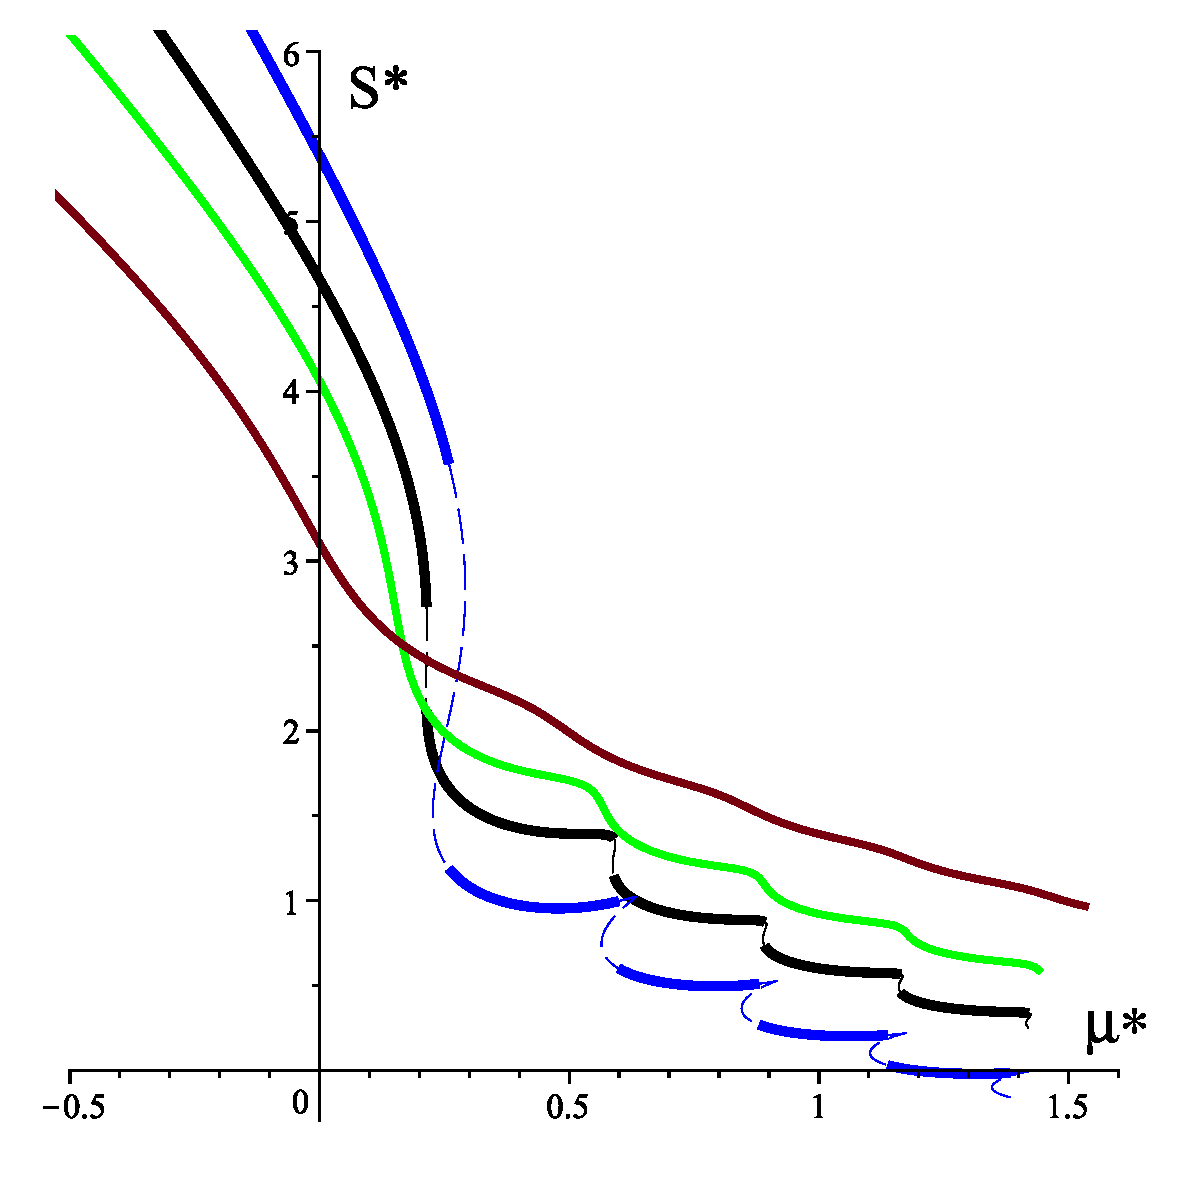
\includegraphics[width=7.0cm]{images/entropy_per_particle_vs_mu3}}
		%\hfill
		%\subfloat[\centering]{
\includegraphics[width=7.0cm]{Definitions/logo-mdpi}}\\
		\subfloat[\centering]{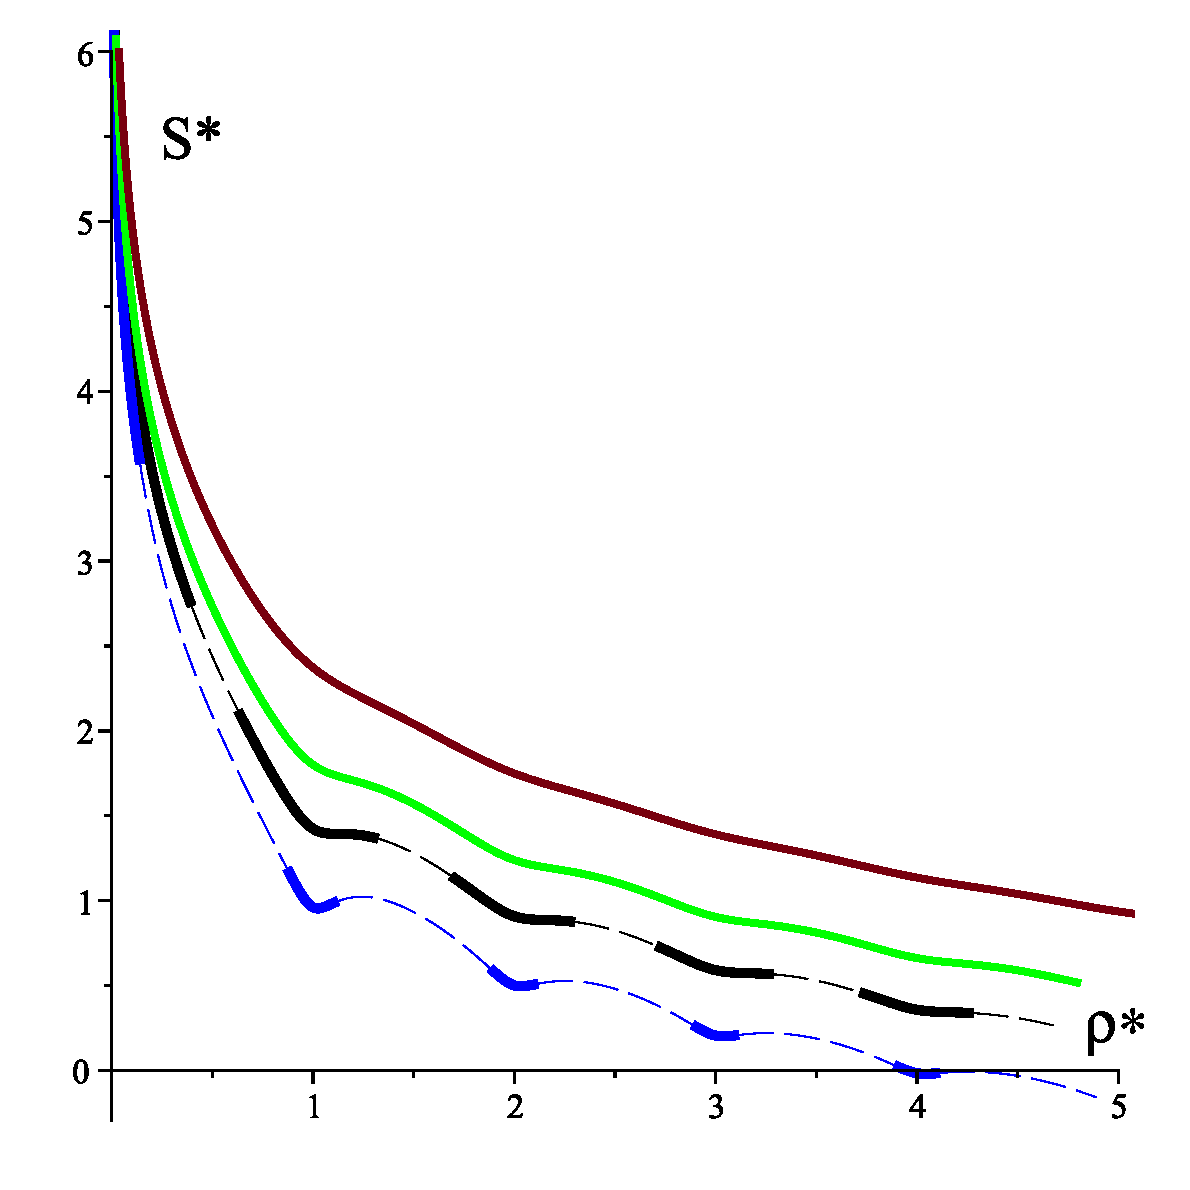
\includegraphics[width=7.0cm]{images/entropy_per_particle_vs_rho3}}\\
		%\subfloat[\centering]{
\includegraphics[width=7.0cm]{Definitions/logo-mdpi}}
		\subfloat[\centering]{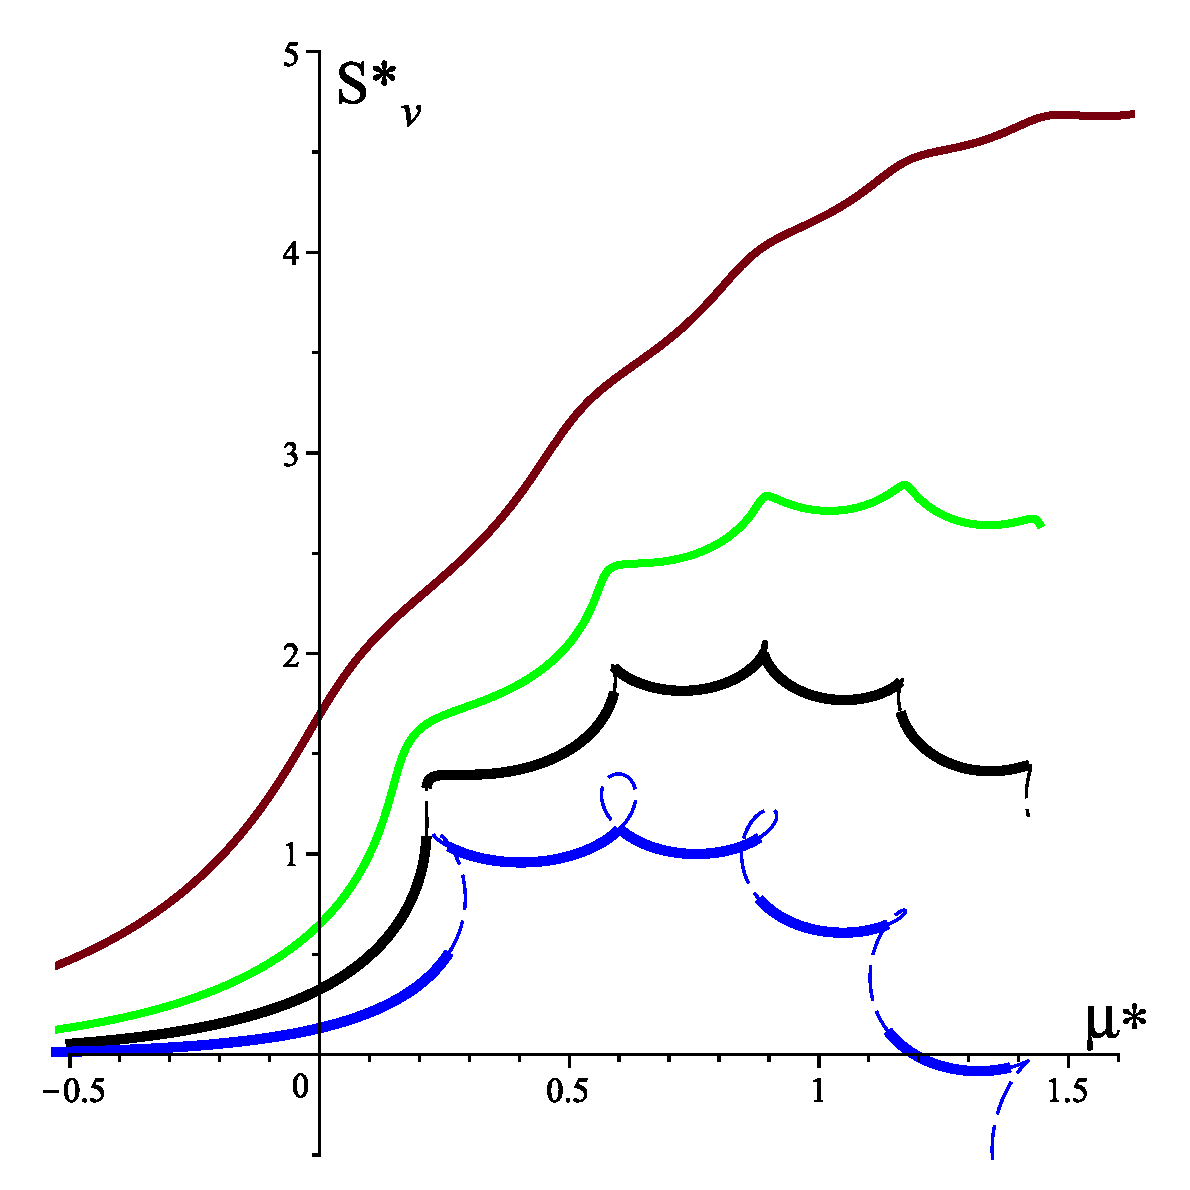
\includegraphics[width=7.0cm]{images/entropy_per_cell_vs_mu4}}
		%\hfill
		%\subfloat[\centering]{
\includegraphics[width=7.0cm]{Definitions/logo-mdpi}}
		\subfloat[\centering]{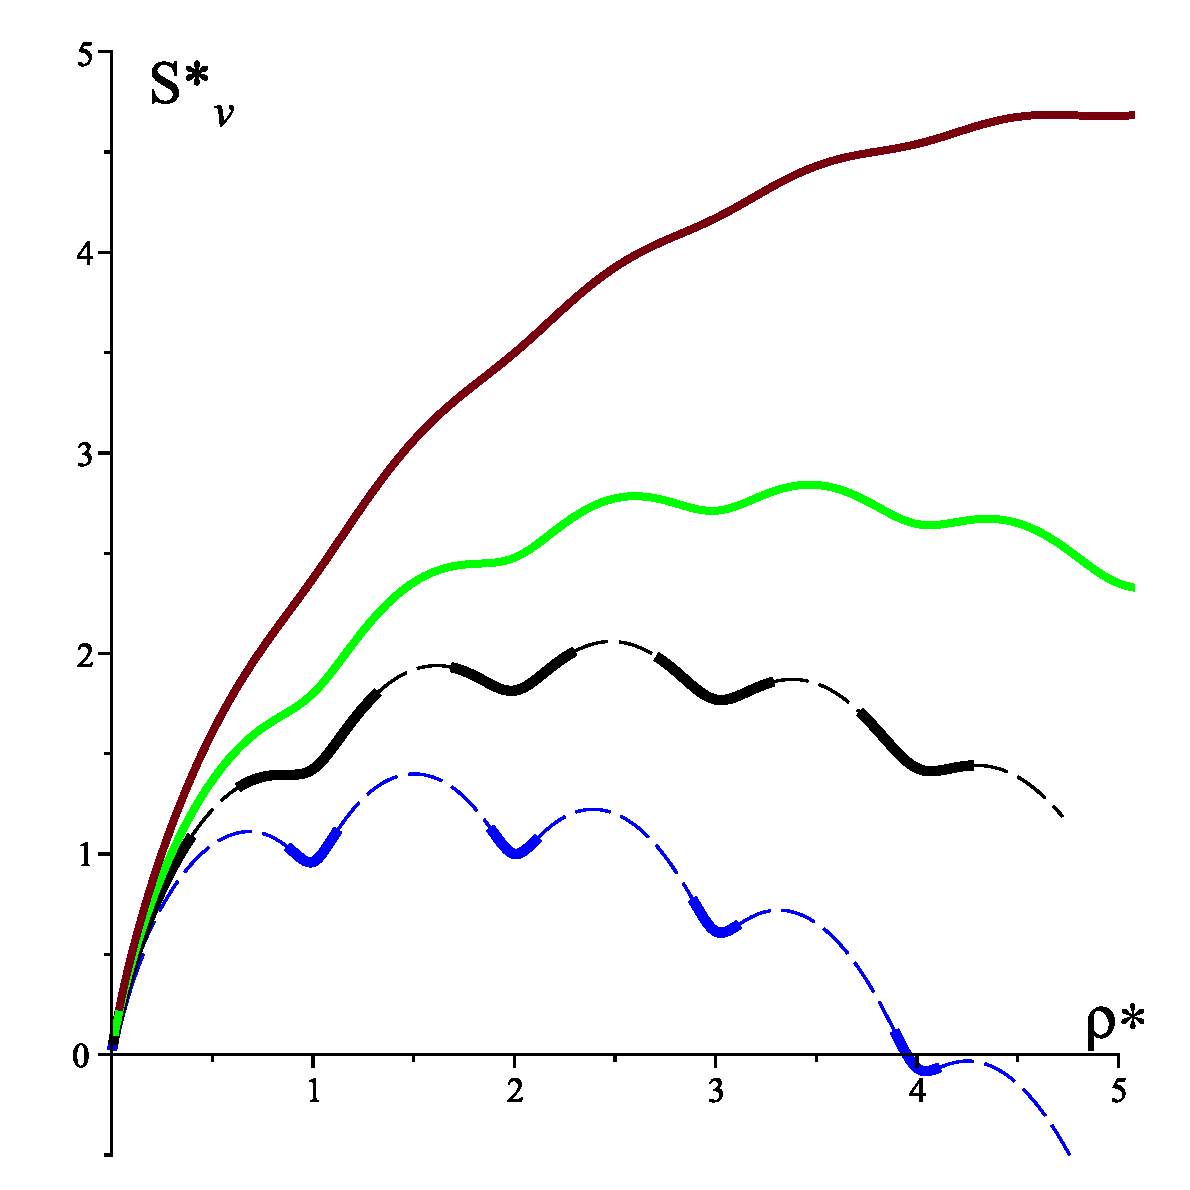
\includegraphics[width=7.0cm]{images/entropy_per_cell_vs_rho4}}
		%\isPreprints{} % If the paper is ``preprints'', please uncomment this parenthesis.
	\caption{Entropy: (\textbf{a}) Entropy per particle versus chemical potential. (\textbf{b}) Entropy per particle versus density. (\textbf{c}) Entropy per cell versus chemical potential. (\textbf{d}) Entropy per cell versus density. In all figures, color curves correspond to the following temperatures: Red - $T^*=0.40$; Green - $T^*=0.30$ Black - $T^*=0.25$; Blue - $T^* = 0.20$. Parameters are takes as $a=1.2$ and $v^*=5.0$.\label{fig:entropy3}}
\end{figure} 

The dependence of the entropy per cell on the chemical potential is illustrated in Figure~\ref{fig:entropy3}(c). At high temperatures, i.e. $T^*=0.4$, the entropy per cell increases as a function of $\mu^*$ for negative and small positive values, then reaches a maximum, and then starts decreasing. For temperatures just slightly above the critical ones, i.e. $T^*=0.3$, the behavior of $S^*_v$ is very nontrivial, with noticeable bends around the approaching critical points. At lower temperatures, the entropy per cell increases with $\mu^*$ in Phase I. In Phase II and Phase III, it has a non-monotonic behavior, but overall, these phases possess the highest entropy per cell compared to all the other phases. Then, for the consecutive phases, the entropy per cell jumps to lower values at each phase transition, while still having non-monotonic behavior within a single phase. 

The dependence of the entropy per cell on the density is presented in Figure~\ref{fig:entropy3}(d). For high temperatures, i.e. $T^*=0.4$, the entropy per cell increases as a function of $\rho^*$ for small values, reaches a maximum, and then starts decreasing. For temperatures just slightly above the critical ones, i.e. $T^*=0.3$, the behavior of $S^*_v$ starts to resemble that below $T_c$, signaling the approach to critical points. At lower temperatures, the entropy per cell increases with $\rho^*$ in Phase I. Then, within each consecutive phase, it exhibits a non-monotonic behavior, and possesses minima at around integer-valued $\rho^*$.
Based on the available data, even though very scarce, we assume that such behavior of the entropy versus density is a generic characteristic of cell (lattice) models allowing for multiple occupancy, see the discussion in the next Section~\ref{sec:dis}.

%%%%%%%%%%%%%%%%%%%%%%%%%%%%%%%%%%%%%%%%%%
\section{Discussion}\label{sec:dis}
Published results on entropy in multiple-occupancy lattice models are scarce. To our knowledge, no analogous results exist for classical systems, while several studies have addressed the quantum cases. Interestingly, these quantum models exhibit features remarkably similar to those found in our classical cell fluid, suggesting a common physical origin -- the allowance for multiple occupancy. 

Study~\citep{dLBKGS11} thoroughly examines both entropy per site and the entropy per cell for the three-dimensional fermionic Hubbard model by the dynamical mean-field theory. In this model, the maximum occupancy (or filling) is 2. Note that their concept of the entropy per site is analogous to our entropy per cell.
The entropy per site as a function of chemical potential is presented in~\citep[Figs.~5 and~6]{dLBKGS11}. The dependence of the entropy per site on density is shown in \citep[Fig.~7]{dLBKGS11}.
That of the entropy per particle on density is illustrated in \citep[Fig.~8]{dLBKGS11}. All Figures contain curves for multiple temperatures, and different Hamiltonian parameters of the considered Hubbard model.
The dependence of the entropy per particle on the chemical potential is absent though. Qualitative similarities between our results and the results of~\citep{dLBKGS11} are as follows. The evolution of the entropy per cell for the cell model as a function of $\mu^*$ at high temperature, i.e. $T^*=0.4$ in Figure~\ref{fig:entropy3}(c), is similar to the entropy per site versus chemical potential for the Hubbard model at the weak interaction strength, cf. Fig.~5 from~\citep{dLBKGS11}. At the low temperature, our result at $T^*=0.3$ resembles that of~\citep[Fig.~6]{dLBKGS11} for the Hubbard model at the strong interaction strength. The similarity is particularly evident in the interval $0.7 \leq \mu^* \leq 1.3$ (Figure~\ref{fig:entropy3}(c), green curve), where two maxima of $S^*_v$ are observed. The behavior of the entropy per cell versus density, Figure~\ref{fig:entropy3}(d), at high temperature, i.e. $T^*=0.4$, is qualitatively the same as the entropy per site versus density of the Hubbard model at the weak interaction strength~\citep[Fig.~7]{dLBKGS11}. At low temperature, the qualitative similarity is observed in the region at $\rho \approx 1.0$, where the dips in the entropy per cell are developed in both models. Finally, we compare the entropy per particle $S^*$, Figure~\ref{fig:entropy3}(b), with that of the Hubbard model from~\citep[Fig.~7]{dLBKGS11}. The high temperature regime in Figure~\ref{fig:entropy3}(b) clearly resembles the weak interaction strength regime in~\citep[Fig.~7]{dLBKGS11}. In turn, at the low temperature regime, $T^*=0.2$, for Phase II, the entropy per particle develops a minima at $\rho^* \approx 1$ analogously as in the Hubbard model at the strong interaction strength~\citep[Fig.~7]{dLBKGS11}.

Results similar to those in Ref.~\citep{dLBKGS11} were also reported in Refs.~\citep{Campo15},~\citep{PKF20}, for the one-dimensional repulsive Hubbard model, studied using different methods. In both studies, see~\citep[Fig.~4]{Campo15} and~\citep[Fig.21a]{PKF20}, the entropy per site exhibits a single maximum at high temperature, and a pronounced minimum at density $\rho^*=1.0$ at low temperature, which is consistent with our results in Figure~\ref{fig:entropy3}. 

In~\citep{PKvHT08} the entropy in the single-band Bose-Hubbard model is studied in one and two dimensions by the quantum Monte Carlo methods. The entropy per site as a function of the filling is presented in \citep[Fig.~2]{PKvHT08} for the homogeneous 1D Bose-Hubbard system. There, the plot is extended up to the value of filling $n = 3.0$, and at the moment, this is the only study we found that reports the dependence of the entropy per site on the average occupancy number for the density exceeding $\rho^* \approx 2.0$. In~\citep[Fig.~2]{PKvHT08}, we observe two dips at fillings $n = 1.0$ and $n = 2.0$, see the red curve for $U/t = 12$. Analogous dips are observed in our model as well, around $\rho^* \approx 1.0$ and $\rho^* \approx 2.0$, respectively, at $T^*=0.2$, see~Figure~\ref{fig:entropy3}(d).

In summary, despite their different physical nature, the allowance for maximum occupancy to be higher than unity leads to outstandingly similar features in the mentioned models. The Hubbard model, allowing for $\rho^*_{\rm max} = 2.0$, develops a minima in the entropy per site at $\rho^* = 1.0$. The Bose-Hubbard model data, reported up to $\rho^* \leq 3.0$ show the minima for the entropy per site at $\rho^*=1.0$ and at $\rho^* = 2.0$. The cell model with the Curie-Weiss interaction considered in the current work does not have any restriction on the occupancy number, and thus develops the minima in the entropy per cell at $\rho^* \approx 1.0$, $\rho^* \approx 2.0$, $\rho^* \approx 3.0$, and so on. We expect this feature to appear in other multiple-occupancy lattice gas models as well. In particular, the entropy per cell in the double-occupancy lattice gas~\citep{LYZ21} should have a dip at $\rho^* = 1.0$. The generalized exponential model of index $4$ considered in \citep{Prestipino14,PGT15} in the context of cluster crystals, and the lattice gas model of multiple layer adsorption~\citep{dOG78} should both have minima in the entropy per site at integer-valued densities as both models exhibit multiple first-order phase transitions at sufficiently low temperatures, similar to the cell model studied by us. The same arguments apply to the entropy per particle as well.

Additionally, in Appendix~\ref{app:vdW}, we present the entropy of the van der Waals fluid, in a form analogous to Figure~\ref{fig:entropy3}. Note, that qualitative comparison between the cell model and the van der Waals theory can be made only for the transition between Phase I and Phase II. This suggests that the first-order phase transition between Phase I and Phase II is of liquid-gas type.


%%%%%%%%%%%%%%%%%%%%%%%%%%%%%%%%%%%%%%%%%%
\section{Conclusions}
\label{sec:conclusions}
We have analytically derived explicit expressions for the entropy of a cell fluid model with multiple occupancy and Curie–Weiss-type interaction. Within this framework, both the entropy per particle and the entropy per cell were obtained as functions of temperature and chemical potential, and their dependences on density were represented in a parametric form. The analysis demonstrates that the entropy exhibits a sequence of discontinuities at first-order phase transitions, in full correspondence with the infinite cascade of coexistence regions between fluid phases of increasing density.

At temperatures below the critical points, the entropy per particle decreases stepwise with increasing chemical potential, while the entropy per cell shows pronounced nonmonotonic behavior within individual phases. In the ``entropy–density'' representation, both quantities display distinct minima near integer-valued densities. These minima are directly related to the discrete character of cell occupancy and appear to be a generic thermodynamic signature of multiple-occupancy lattice systems.

The study further reveals that, at sufficiently high densities or small values of the reduced cell volume $v^*$, the entropy may become negative, which is an artifact of the classical treatment analogous to that observed in the Gaussian-core model. Increasing $v^*$ shifts this behavior to higher densities while preserving the overall qualitative pattern.

A qualitative comparison with lattice models of different microscopic origin, such as the fermionic Hubbard, and Bose–Hubbard models, shows that all systems allowing for more than single occupancy develop entropy minima at integer densities. The present Curie–Weiss cell model, unrestricted in occupancy number, extends this tendency to an infinite sequence of minima corresponding to each successive phase. This feature suggests a unifying thermodynamic behavior among multiple-occupancy lattice gases (cell fluids) and related soft-matter systems with cluster-forming interactions.

%%%%%%%%%%%%%%%%%%%%%%%%%%%%%%%%%%%%%%%%%%
\vspace{6pt} 

%%%%%%%%%%%%%%%%%%%%%%%%%%%%%%%%%%%%%%%%%%
\authorcontributions{}

\funding{This work was supported by the National Research Foundation of Ukraine under the project No. 2023.03/0201.}

\dataavailability{} 

\acknowledgments{}

\conflictsofinterest{The authors declare no conflicts of interest.} 

%%%%%%%%%%%%%%%%%%%%%%%%%%%%%%%%%%%%%%%%%%
%% Optional

%% Only for journal Encyclopedia
%\entrylink{The Link to this entry published on the encyclopedia platform.}

\abbreviations{Abbreviations}{
The following abbreviations are used in this manuscript:
\\

\noindent 
\begin{tabular}{@{}ll}
MDPI & Multidisciplinary Digital Publishing Institute\\
GPF & Grand partition function\\
\end{tabular}
}

%%%%%%%%%%%%%%%%%%%%%%%%%%%%%%%%%%%%%%%%%%
%% Optional
\appendixtitles{no} % Leave argument "no" if all appendix headings stay EMPTY (then no dot is printed after "Appendix A"). If the appendix sections contain a heading then change the argument to "yes".
\appendixstart
\appendix
\section[\appendixname~\thesection]{Entropy in the van der Waals fluid}
\label{app:vdW}

The entropy of the van der Waals (vdW) fluid is expressed via density and temperature as~\citep[(55)]{Johnston14}
\begin{equation}
	\label{vdw:S}
	\frac{S}{N k_{\rm B}} = \ln \left[x_c\hat{\tau}^{3/2}(3-\hat{n})/\hat{n}\right] + \frac{5}{2},
\end{equation}
where $\hat{\tau} = T/T_c$, $\hat{n} = \rho/\rho_c$, and 
\begin{equation}
	x_c \equiv \frac{k_{\rm B} T_c}{8P_c \Lambda^3_c} = \frac{b}{\Lambda^3_c},
\end{equation}
where $\Lambda_c$ is the de Broglie wavelength at the critical temperature, and $b$ is the ``excluded volume'' parameter of the van der Waals theory. The meaning of $b/\Lambda^3_c$ is similar to the meaning of quantity $v^*$ in our cell theory.

\begin{figure}[H]
	%\isPreprints{} % If the paper is ``preprints'', please uncomment this parenthesis.
		%\subfloat[\centering]{
\includegraphics[width=7.0cm]{Definitions/logo-mdpi}}
		\subfloat[\centering]{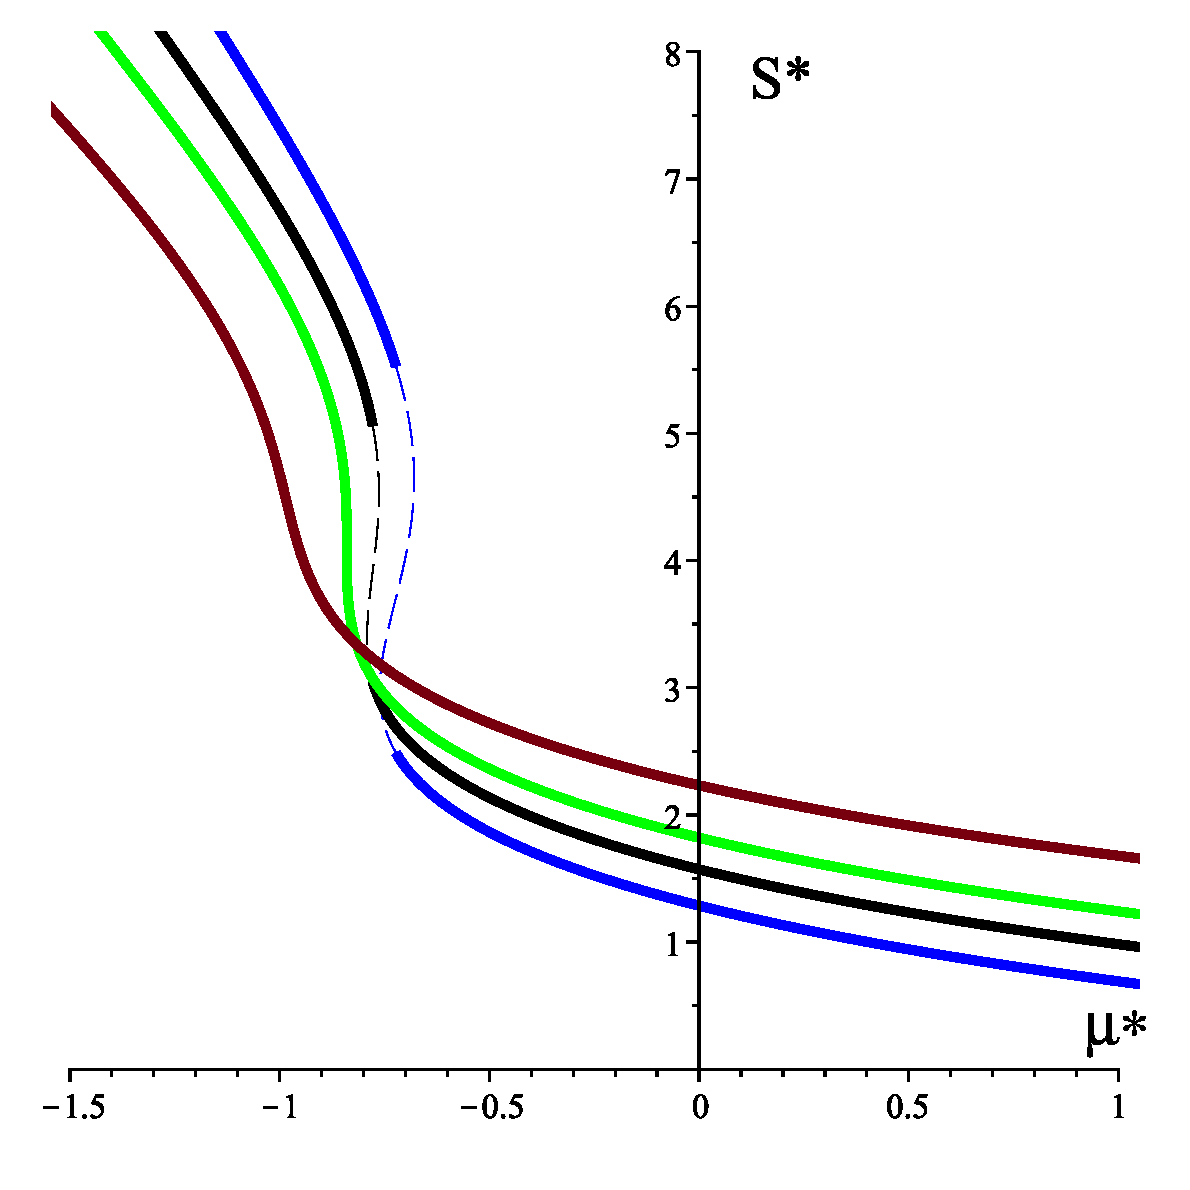
\includegraphics[width=6.0cm]{images/vdW/entropy_per_particle_vs_mu_vdW}}
		%\hfill
		%\subfloat[\centering]{
\includegraphics[width=7.0cm]{Definitions/logo-mdpi}}\\
		\subfloat[\centering]{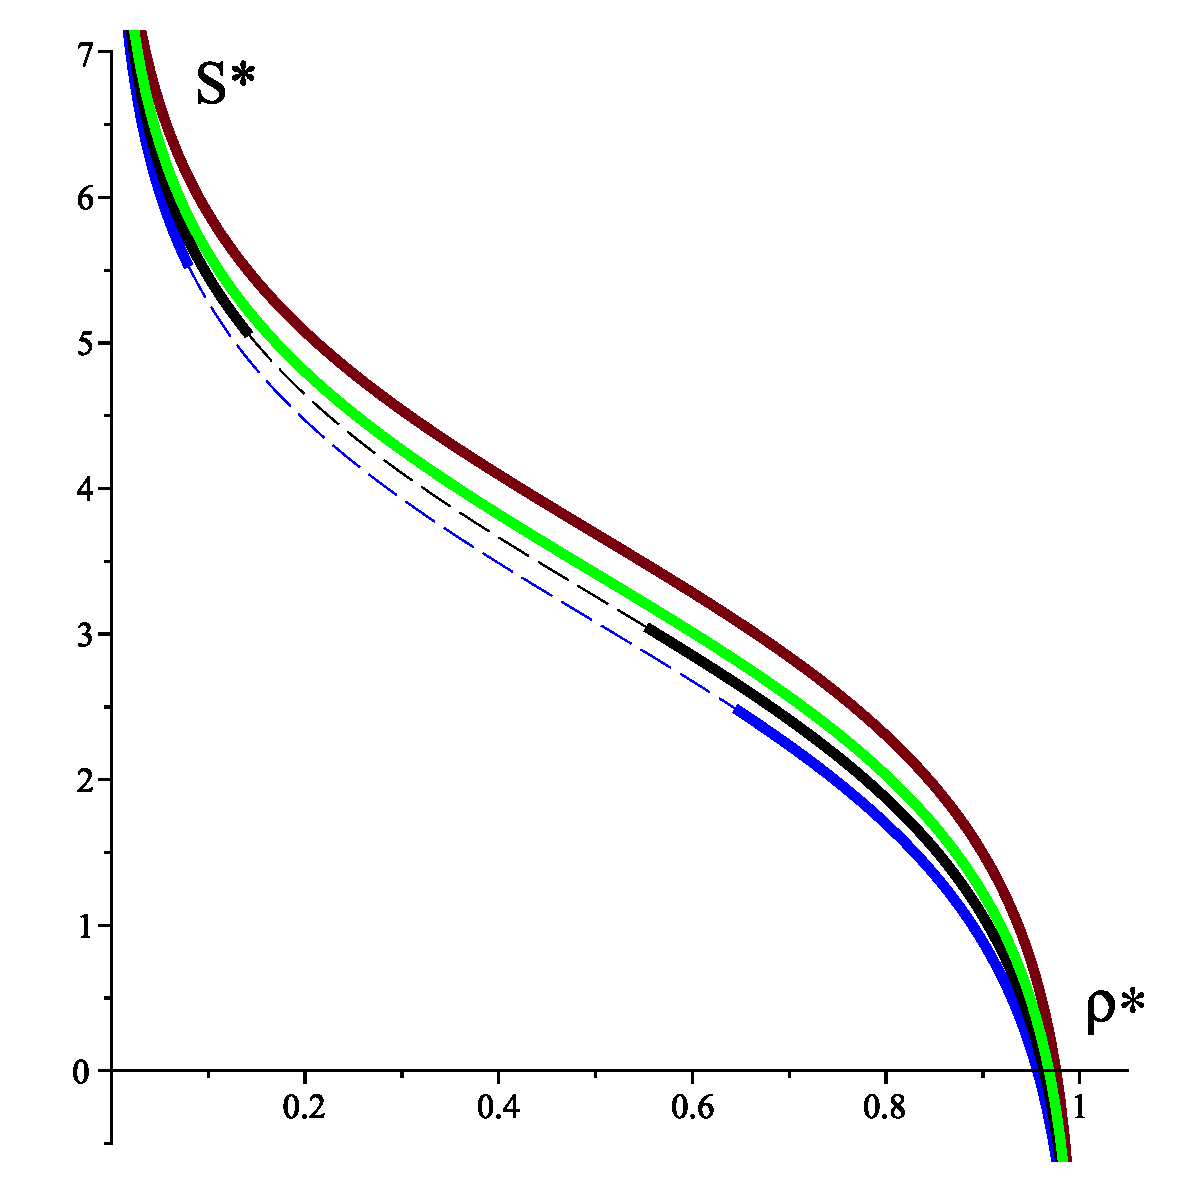
\includegraphics[width=6.0cm]{images/vdW/entropy_per_particle_vs_rho_vdW}}\\
		%\subfloat[\centering]{
\includegraphics[width=7.0cm]{Definitions/logo-mdpi}}
		\subfloat[\centering]{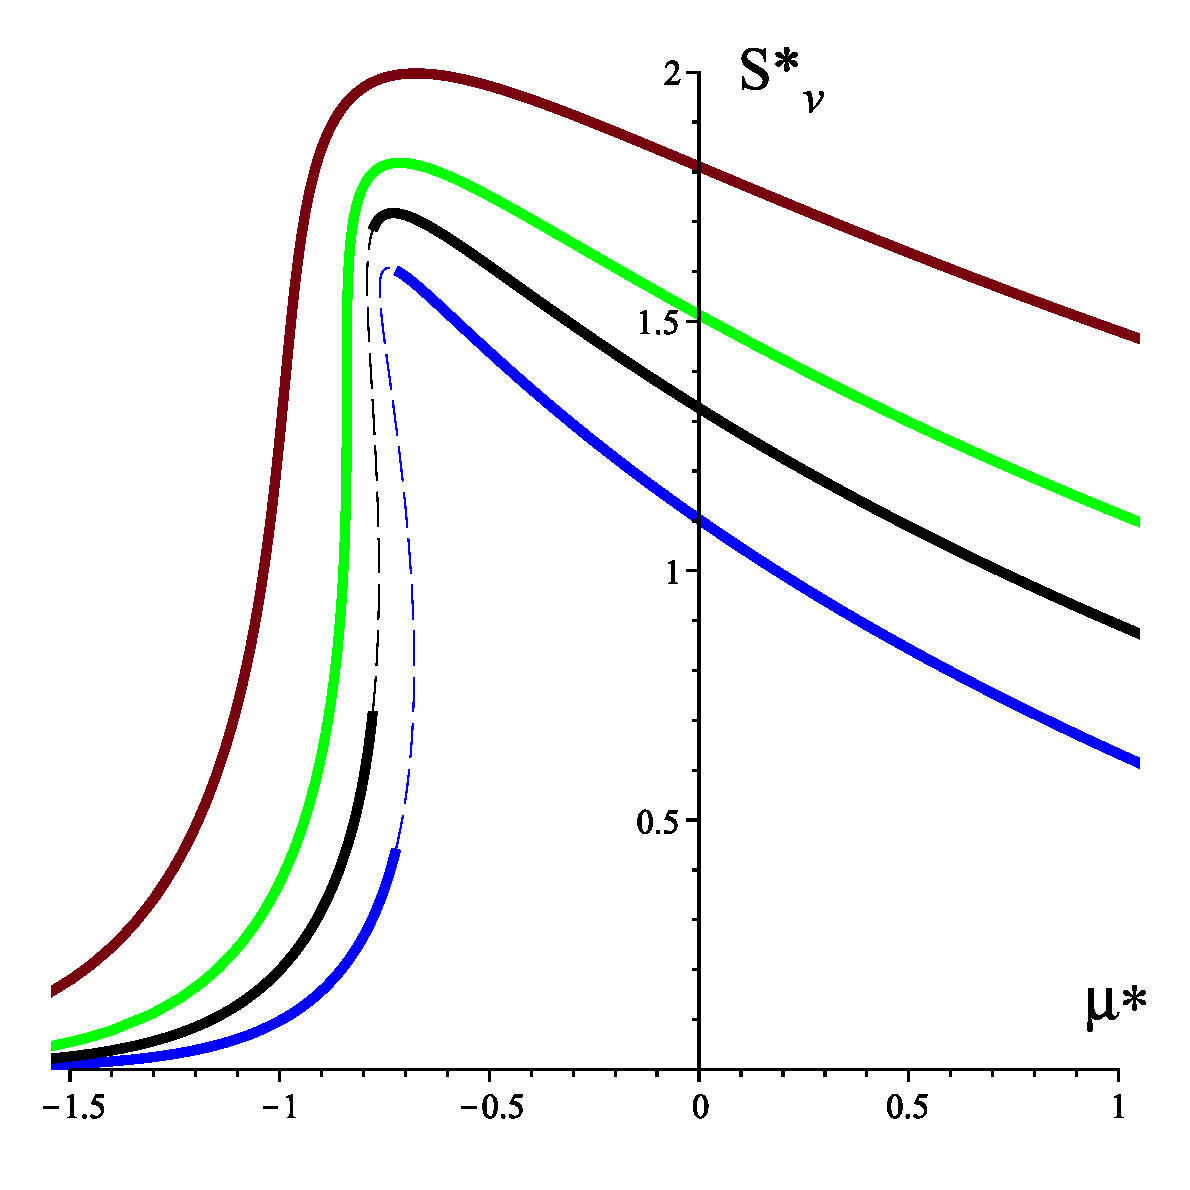
\includegraphics[width=6.0cm]{images/vdW/entropy_per_cell_vs_mu_vdW}}
		%\hfill
		%\subfloat[\centering]{
\includegraphics[width=7.0cm]{Definitions/logo-mdpi}}
		\subfloat[\centering]{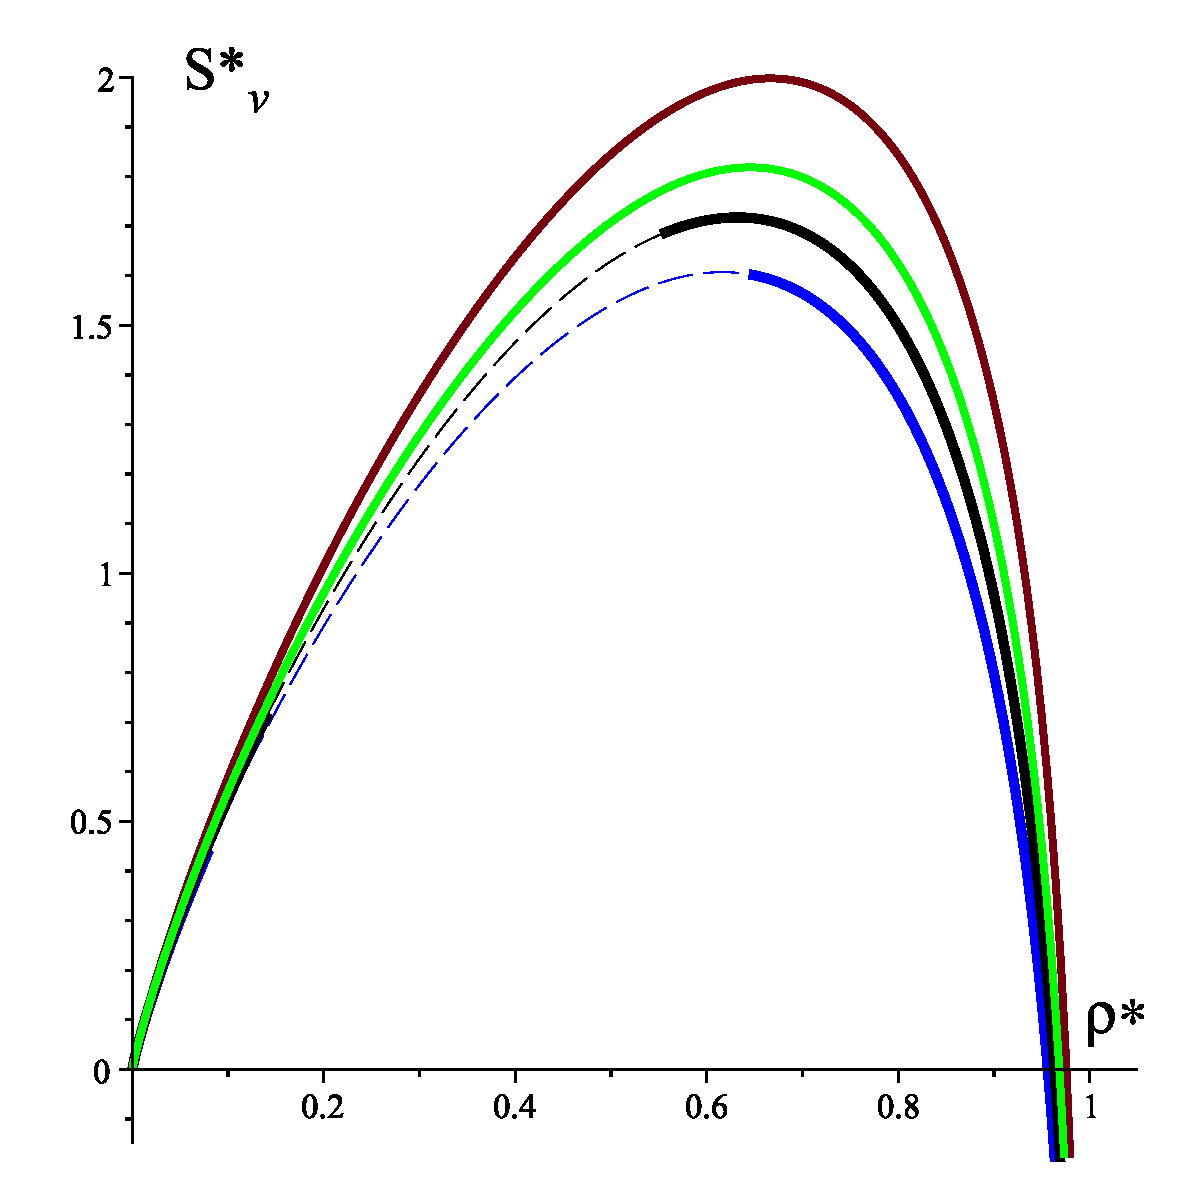
\includegraphics[width=6.0cm]{images/vdW/entropy_per_cell_vs_rho_vdW}}
		%\isPreprints{} % If the paper is ``preprints'', please uncomment this parenthesis.
	\caption{Entropy of the van der Waals fluid: (\textbf{a}) Entropy per particle versus chemical potential. (\textbf{b}) Entropy per particle versus density. (\textbf{c}) Entropy per cell versus chemical potential. (\textbf{d}) Entropy per cell versus density. In all figures, color curves correspond to the following temperatures: Red - $T^*_{\mathrm{vdW}}=0.0.3$; Green - $T^*_{\mathrm{vdW}}=0.25$ Black - $T^*_{\mathrm{vdW}}=0.225$; Blue - $T^*_{\mathrm{vdW}} = 0.20$. The value of the parameter: $v^*_{\mathrm{vdW}}=5.0$.\label{fig:entropy_vdW}}
\end{figure} 

The chemical potential of the vdW fluid as a function of temperature and density is given by~\cite[(70c)]{Johnston14}
\begin{equation}
	\label{vdw:mu}
	\frac{\mu}{k_{\rm B}T_c} = -\hat{\tau} \ln \left(\frac{3-\hat{n}}{\hat{n}}\right) + \frac{\hat{\tau}\hat{n}}{3-\hat{n}} - \frac{9\hat{n}}{4} - \hat{\tau}\ln(\hat{\tau}^{3/2}) - \hat{\tau}\ln(x_c).
\end{equation}
Eqs.~\eqref{vdw:mu} and~\eqref{vdw:S} can be considered as a parametric equation for the entropy as a function of the chemical potential, with density $\hat{n}$ being the parameter.

In Fig.~\ref{fig:entropy_vdW}, the behavior of the entropy in the van der Waals fluid is demonstrated in terms of the appropriate reduced variables:
\begin{equation}
	\rho^*_{\mathrm{vdW}} = \frac{\hat{n}}{3}; \quad T^*_{vdW} = \frac{\hat{\tau}}{4}; \quad \mu^*_{vdW} = \frac{\mu}{4k_{\mathrm B}T_c}
\end{equation}
Note, that in such representation, $v^*_{\mathrm{vdW}} = 2x_c$.

In the van der Waals theory, the concept of entropy per cell is formally meant as the product of the entropy per particle $S^*_{\mathrm{vdW}}$ and density $\rho^*_{\mathrm{vdW}}$, by analogy with the cell model.




%%%%%%%%%%%%%%%%%%%%%%%%%%%%%%%%%%%%%%%%%%
%\isPreprints{} % If the paper is ``preprints'', please uncomment this parenthesis.
%\printendnotes[custom] % Un-comment to print a list of endnotes

\reftitle{References}

% Please provide either the correct journal abbreviation (e.g. according to the “List of Title Word Abbreviations” http://www.issn.org/services/online-services/access-to-the-ltwa/) or the full name of the journal.
% Citations and References in Supplementary files are permitted provided that they also appear in the reference list here. 

%=====================================
% References, variant A: external bibliography
%=====================================
\bibliography{articles,books}

%=====================================
% References, variant B: internal bibliography
%=====================================

% ACS format
%\isAPAandChicago{}{%
%\begin{thebibliography}{999}
%% Reference 1
%\bibitem[Author1(year)]{ref-journal}
%Author~1, T. The title of the cited article. {\em Journal Abbreviation} {\bf 2008}, {\em 10}, 142--149.
%% Reference 2
%\bibitem[Author2(year)]{ref-book1}
%Author~2, L. The title of the cited contribution. In {\em The Book Title}; Editor 1, F., Editor 2, A., Eds.; Publishing House: City, Country, 2007; pp. 32--58.
%% Reference 3
%\bibitem[Author1 and Author2 (year)]{ref-book2}
%Author 1, A.; Author 2, B. \textit{Book Title}, 3rd ed.; Publisher: Publisher Location, Country, 2008; pp. 154--196.
%% Reference 4
%\bibitem[Author4(year)]{ref-unpublish}
%Author 1, A.B.; Author 2, C. Title of Unpublished Work. \textit{Abbreviated Journal Name} year, \textit{phrase indicating stage of publication (submitted; accepted; in press)}.
%% Reference 5
%\bibitem[Author8(year)]{ref-url}
%Title of Site. Available online: URL (accessed on Day Month Year).
%% Reference 6
%\bibitem[Author6(year)]{ref-proceeding}
%Author 1, A.B.; Author 2, C.D.; Author 3, E.F. Title of presentation. In Proceedings of the Name of the Conference, Location of Conference, Country, Date of Conference (Day Month Year); Abstract Number (optional), Pagination (optional).
%% Reference 7
%\bibitem[Author7(year)]{ref-thesis}
%Author 1, A.B. Title of Thesis. Level of Thesis, Degree-Granting University, Location of University, Date of Completion.
%\end{thebibliography}
%}

% Chicago format (Used for journal: arts, genealogy, histories, humanities, jintelligence, laws, literature, religions, risks, socsci)
%\isChicagoStyle{%
%\begin{thebibliography}{999}
%% Reference 1
%\bibitem[Aranceta-Bartrina(1999a)]{ref-journal}
%Aranceta-Bartrina, Javier. 1999a. Title of the cited article. \textit{Journal Title} 6: 100--10.
%% Reference 2
%\bibitem[Aranceta-Bartrina(1999b)]{ref-book1}
%Aranceta-Bartrina, Javier. 1999b. Title of the chapter. In \textit{Book Title}, 2nd ed. Edited by Editor 1 and Editor 2. Publication place: Publisher, vol. 3, pp. 54–96.
%% Reference 3
%\bibitem[Baranwal and Munteanu {[1921]}(1955)]{ref-book2}
%Baranwal, Ajay K., and Costea Munteanu. 1955. \textit{Book Title}. Publication place: Publisher, pp. 154--96. First published 1921 (op-tional).
%% Reference 4
%\bibitem[Berry and Smith(1999)]{ref-thesis}
%Berry, Evan, and Amy M. Smith. 1999. Title of Thesis. Level of Thesis, Degree-Granting University, City, Country. Identifi-cation information (if available).
%% Reference 5
%\bibitem[Cojocaru et al.(1999)]{ref-unpublish}
%Cojocaru, Ludmila, Dragos Constatin Sanda, and Eun Kyeong Yun. 1999. Title of Unpublished Work. \textit{Journal Title}, phrase indicating stage of publication.
%% Reference 6
%\bibitem[Driver et al.(2000)]{ref-proceeding}
%Driver, John P., Steffen Rohrs, and Sean Meighoo. 2000. Title of Presentation. In \textit{Title of the Collected Work} (if available). Paper presented at Name of the Conference, Location of Conference, Date of Conference.
%% Reference 7
%\bibitem[Harwood(2008)]{ref-url}
%Harwood, John. 2008. Title of the cited article. Available online: URL (accessed on Day Month Year).
%\end{thebibliography}
%}{}

% APA format (Used for journal: admsci, behavsci, businesses, econometrics, economies, education, ejihpe, games, humans, ijfs, journalmedia, jrfm, languages, psycholint, publications, tourismhosp, youth)
%\isAPAStyle{%
%\begin{thebibliography}{999}
%% Reference 1
%\bibitem[\protect\citeauthoryear{Azikiwe \BBA\ Bello}{{2020a}}]{ref-journal}
%Azikiwe, H., \& Bello, A. (2020a). Title of the cited article. \textit{Journal Title}, \textit{Volume}(Issue), 
%Firstpage--Lastpage/Article Number.
%% Reference 2
%\bibitem[\protect\citeauthoryear{Azikiwe \BBA\ Bello}{{2020b}}]{ref-book1}
%Azikiwe, H., \& Bello, A. (2020b). \textit{Book title}. Publisher Name.
%% Reference 3
%\bibitem[Davison(1623/2019)]{ref-book2}
%Davison, T. E. (2019). Title of the book chapter. In A. A. Editor (Ed.), \textit{Title of the book: Subtitle} 
%(pp. Firstpage--Lastpage). Publisher Name. (Original work published 1623) (Optional).
%% Reference 4
%\bibitem[Fistek et al.(2017)]{ref-proceeding}
%Fistek, A., Jester, E., \& Sonnenberg, K. (2017, Month Day). Title of contribution [Type of contribution]. Conference Name, Conference City, Conference Country.
%% Reference 5
%\bibitem[Hutcheson(2012)]{ref-thesis}
%Hutcheson, V. H. (2012). \textit{Title of the thesis} [XX Thesis, Name of Institution Awarding the Degree].
%% Reference 6
%\bibitem[Lippincott \& Poindexter(2019)]{ref-unpublish}
%Lippincott, T., \& Poindexter, E. K. (2019). \textit{Title of the unpublished manuscript} [Unpublished manuscript/Manuscript in prepara-tion/Manuscript submitted for publication]. Department Name, Institution Name.
%% Reference 7
%\bibitem[Harwood(2008)]{ref-url}
%Harwood, J. (2008). \textit{Title of the cited article}. Available online: URL (accessed on Day Month Year).
%\end{thebibliography}
%}{}

% If authors have biography, please use the format below
%\section*{Short Biography of Authors}
%\bio
%{\raisebox{-0.35cm}{\includegraphics[width=3.5cm,height=5.3cm,clip,keepaspectratio]{Definitions/author1.pdf}}}
%{\textbf{Firstname Lastname} Biography of first author}
%
%\bio
%{\raisebox{-0.35cm}{\includegraphics[width=3.5cm,height=5.3cm,clip,keepaspectratio]{Definitions/author2.jpg}}}
%{\textbf{Firstname Lastname} Biography of second author}

% For the MDPI journals use author-date citation, please follow the formatting guidelines on http://www.mdpi.com/authors/references
% To cite two works by the same author: \citeauthor{ref-journal-1a} (\citeyear{ref-journal-1a}, \citeyear{ref-journal-1b}). This produces: Whittaker (1967, 1975)
% To cite two works by the same author with specific pages: \citeauthor{ref-journal-3a} (\citeyear{ref-journal-3a}, p. 328; \citeyear{ref-journal-3b}, p.475). This produces: Wong (1999, p. 328; 2000, p. 475)

%%%%%%%%%%%%%%%%%%%%%%%%%%%%%%%%%%%%%%%%%%
%% for journal Sci
%\reviewreports{\\
%Reviewer 1 comments and authors’ response\\
%Reviewer 2 comments and authors’ response\\
%Reviewer 3 comments and authors’ response
%}
%%%%%%%%%%%%%%%%%%%%%%%%%%%%%%%%%%%%%%%%%%
\PublishersNote{}
%\isPreprints{} % If the paper is ``preprints'', please uncomment this parenthesis.
\end{document}

We derived analytical expressions for the entropy of the cell fluid model with multiple occupancy and Curie–Weiss-type interaction. The obtained formulas describe the entropy per particle and per cell as functions of temperature, chemical potential, and density. The results show that at low temperatures the entropy changes discontinuously at first-order phase transitions and forms a sequence of steps between fluid phases of increasing density. In the entropy–density plane, both quantities have clear minima near integer densities. This behavior is a characteristic feature of models that allow several particles in one cell. At very high densities, the entropy becomes negative, which is a consequence of the classical approximation. The same type of entropy minima is also found in the Hubbard and Bose–Hubbard models, showing that the presence of multiple occupancy leads to similar thermodynamic features in different lattice systems.
